% Apêndice A: tabela hash com encadeamento separado (m = 7, h(k) = k % 7).
\documentclass[border=4pt]{standalone}
\usepackage[utf8]{inputenc}
\usepackage[T1]{fontenc}
% Estilo comum das figuras de listas (incluído pelas figuras dos capítulos 3 e 4).
\usepackage{tikz}
\usetikzlibrary{arrows.meta, positioning, shapes.multipart, calc}
\definecolor{navy}{RGB}{23,45,80}
\definecolor{laranja}{RGB}{250,110,29}
\definecolor{cinzalogo}{RGB}{107,114,126}
\tikzset{
  no/.style={rectangle split, rectangle split horizontal, rectangle split parts=2,
             draw=navy, line width=0.9pt, minimum height=7mm,
             rectangle split part fill={laranja!15, white}, font=\sffamily\small},
  no3/.style={rectangle split, rectangle split horizontal, rectangle split parts=3,
              draw=navy, line width=0.9pt, minimum height=7mm,
              rectangle split part fill={white, laranja!15, white}, font=\sffamily\small},
  seta/.style={-{Stealth[length=2.2mm]}, navy, line width=0.9pt},
  setanova/.style={-{Stealth[length=2.2mm]}, laranja, line width=1.3pt},
  rotulo/.style={font=\sffamily\small\bfseries, text=navy},
  nulo/.style={font=\sffamily\scriptsize, text=cinzalogo},
  passo/.style={font=\sffamily\small, text=cinzalogo, anchor=west},
  legenda/.style={font=\sffamily\scriptsize, text=cinzalogo},
}
% seta que sai do meio da caixa do ponteiro (última parte do nó), na horizontal
\newcommand{\liga}[3][seta]{\draw[#1] ([xshift=-2.3mm]#2.east) -- #3;}

\tikzset{
  balde/.style={draw=navy, line width=0.9pt, minimum width=9mm, minimum height=7mm,
                font=\sffamily\small, fill=white},
  indice/.style={font=\sffamily\scriptsize, text=cinzalogo},
}
\begin{document}
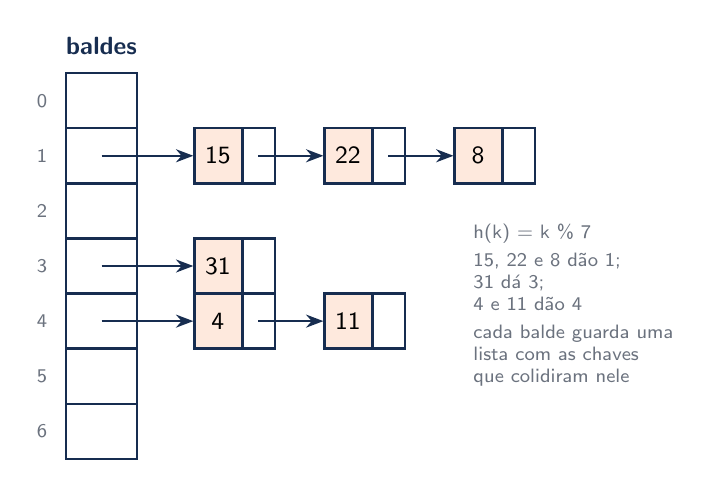
\begin{tikzpicture}
  \foreach \i in {0,...,6} {
    \node[balde] (b\i) at (0, -\i*0.7) {};
    \node[indice, left=1mm of b\i] {\i};
  }
  \node[rotulo, above=1mm of b0] {baldes};
  % balde 1: 15 -> 22 -> 8
  \node[no, right=7mm of b1] (n15) {\makebox[1.1em]{15} \nodepart{two} \phantom{0}};
  \node[no, right=6mm of n15] (n22) {\makebox[1.1em]{22} \nodepart{two} \phantom{0}};
  \node[no, right=6mm of n22] (n8) {\makebox[1.1em]{8} \nodepart{two} \phantom{0}};
  \draw[seta] (b1.center) -- (n15.west);
  \liga{n15}{(n22.west)}
  \liga{n22}{(n8.west)}
  % balde 3: 31
  \node[no, right=7mm of b3] (n31) {\makebox[1.1em]{31} \nodepart{two} \phantom{0}};
  \draw[seta] (b3.center) -- (n31.west);
  % balde 4: 4 -> 11
  \node[no, right=7mm of b4] (n4) {\makebox[1.1em]{4} \nodepart{two} \phantom{0}};
  \node[no, right=6mm of n4] (n11) {\makebox[1.1em]{11} \nodepart{two} \phantom{0}};
  \draw[seta] (b4.center) -- (n4.west);
  \liga{n4}{(n11.west)}
  \node[legenda, align=left, anchor=west] at (4.6, -2.6)
    {h(k) = k \% 7\\[2pt]
     15, 22 e 8 dão 1;\\31 dá 3;\\4 e 11 dão 4\\[2pt]
     cada balde guarda uma\\lista com as chaves\\que colidiram nele};
\end{tikzpicture}
\end{document}
